\chapter{Standard-Plugins}
\index{Plugins|(}
\index{Testerbot}
Die Installation von \xirp~enth�lt die n�tigen Profildateien f�r den
\seegls{Testerbot}. Ebenfalls werden einige Plugins mitgeliefert, die f�r den \seegls{Testerbot}
ben�tigt werden. In diesem Kapitel werden diese Plugins vorgestellt und n�her
beschrieben. Des Weiteren werden einige Kommunikationsplugins mitgeliefert, z.B.
ein Plugin f�r Kommunikation �ber die serielle Schnittstelle.

\newpage

\section{Hallo Welt!}
Das \enquote{Hallo Welt!} Plugin ist das erste Plugin, dass je f�r
\xirp~entwickelt wurde. In seiner momentanen Version ist dieses Plugin
ohne graphische Oberfl�che. Es wird mittels seines Men�eintrages \texttt{Plugins
--> Hallo Welt!} gestartet und gibt in der Systemprotokollansicht einen in den
Einstellungen �nderbaren Text an. Der Standardtext ist \enquote{Hallo Welt!}.
Diese Funktion kann ebenfalls mit dem vom Plugin erzeugten Werkzeugicon
aufgerufen werden. Das \seegls{Icon} ist gekennzeichnet durch ein Puzzelteilbild.

\section{Testerbot Report}
Dieses Plugin zeigt die Funktionsweise von Report-Plugins. Es erzeugt, bei Aufruf
�ber den entsprechenden Men�eintrag (\texttt{Reporte --> Testerbot Report}),
einen Report der die �bertragenen Textnachrichten darstellt.

\section{Thermopile}
\index{Thermopile}
\index{Temperatur}
Dieses \seegls{Sensor}-Plugin zeigt die von einem \seegls{Thermopile}-Array gelieferten W�rmewerte
an. Es zeigt die gemessene Temperatur farblich markiert an. Eine
Farb-Temperaturskala ist unter dem Anzeigebereich angezeigt. In Abbildung
\ref{img:plugins:thermo} auf Seite \pageref{img:plugins:thermo} ist das Plugin in
Aktion zu sehen.

\begin{figure}[ht]
	\centering
	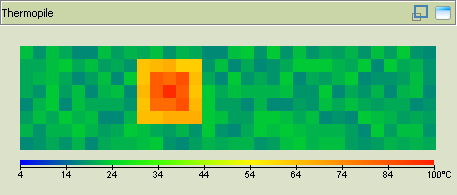
\includegraphics[width=.75\textwidth]{images/thermo}
	\caption{Das Thermopile-Array-Plugin}
	\label{img:plugins:thermo}
\end{figure}

\section{Distanz}
\index{Abstandssensor}
\index{Roboterprofil}
Dieses Plugin zeigt die Werte von Abstandssensoren an. Dieses Plugin bezieht die
Informationen �ber Anzahl und Wertebereich der \seegls{Sensor}en aus dem Roboterprofil. 
In Abbildung \ref{img:plugins:distanz} auf Seite \pageref{img:plugins:distanz}
ist das Plugin in Aktion zu sehen.

\begin{figure}[ht]
	\centering
	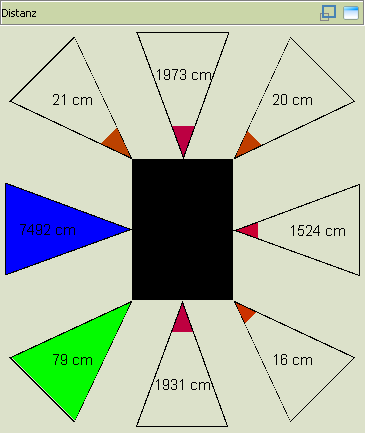
\includegraphics[width=.4\textwidth]{images/distanz}
	\caption{Das Distanz-Plugin}
	\label{img:plugins:distanz}
\end{figure}

\index{Abstandssensor!Infrarot}
\index{Abstandssensor!Ultraschall}
\index{Roboterprofil}
Infratorsensoren werden farblich anders dargestellt als Ultraschallsensoren.
Infratorsensoren werden gr�n und Ultraschallsensoren blau dargestellt, wenn der
Entfernungswert gr��er oder gleich dem Maximum des \seegls{Sensor}s entspricht. Die Farbe
der Sensoranzeigen variiert mit den sich ver�ndernden Werten. Die Einheit in der
die Werte angezeigt werden, werden ebenfalls aus dem Roboterprofil ausgelesen.

\section{Temperatur}
\index{Temperatur}
\index{Thermometer}
\index{Roboterprofil}
Das Temperatur-Plugin zeigt die Werte eines W�rmesensors in Form eines
Thermometers an. Die Markierungen f�r den gelben und roten Bereich erh�lt das
Plugin aus dem Roboterprofil. Die Einheit in der der Wert angezeigt wird, wird
ebenfalls aus dem Roboterprofil ausgelesen. In Abbildung
\ref{img:plugins:temperatur} auf Seite
\pageref{img:plugins:temperatur} ist das Plugin in Aktion zu sehen.

\begin{figure}[htp]
	\centering
	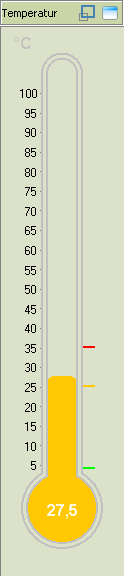
\includegraphics[width=.2\textwidth]{images/temperatur}
	\caption{Das Temperatur-Plugin}
	\label{img:plugins:temperatur}
\end{figure}

\section{CO$_2$}
\index{Kohlendioxid}
\index{CO$_2$}
Dieses \seegls{Sensor}-Plugin zeigt den Verlauf der Werte eines CO$_2$-Sensors an, um so
einen Anstieg des Gases in der umgebenen Luft erkennen zu k�nnen. In Abbildung
\ref{img:plugins:co2} auf Seite \pageref{img:plugins:co2} ist das Plugin in
Aktion zu sehen.

\begin{figure}[ht]
	\centering
	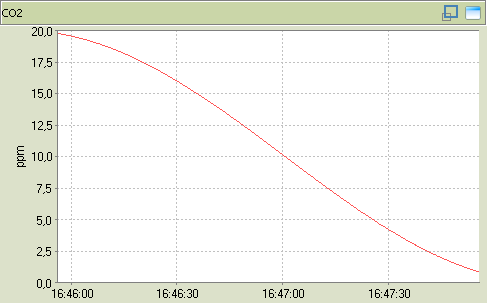
\includegraphics[width=.6\textwidth]{images/co2}
	\caption{Das CO$_2$-Plugin}
	\label{img:plugins:co2}
\end{figure}

\section{Kompass}
\index{Kompass}
\index{Himmelsrichtung}
Das Kompass-Plugin zeigt die aktuell gemessene Himmelsrichtung eines
Kompasssensors in Form eines Kompasses an. Die rote Nadelspitze zeigt die
gemessene Richtung an. In Abbildung \ref{img:plugins:kompass} auf Seite
\pageref{img:plugins:kompass} ist das Plugin in Aktion zu sehen.

\begin{figure}[ht]
	\centering
	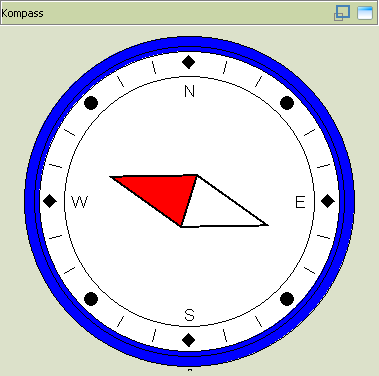
\includegraphics[width=.4\textwidth]{images/kompass}
	\caption{Das Kompass-Plugin}
	\label{img:plugins:kompass}
\end{figure}

\section{Geschwindigkeit}
\index{Geschwindigkeit}
\index{Tachometer}
Dieses Plugin zeigt die gemessene Geschwindigkeit eines Roboters in Form eines
Tachometers an. Die Einheit in der der Wert angezeigt wird, wird
aus dem Roboterprofil ausgelesen. In Abbildung \ref{img:plugins:speed} auf Seite
\pageref{img:plugins:speed} ist das Plugin in Aktion zu sehen.

\begin{figure}[htp]
	\centering
	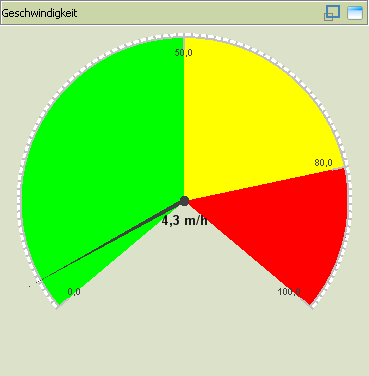
\includegraphics[width=.4\textwidth]{images/speed}
	\caption{Das Geschwindigkeits-Plugin}
	\label{img:plugins:speed}
\end{figure}

\section{Neigung}
\index{Neigung}
\index{Gyroskop}
Dieses Plugin zeigt die gemessenen Werte eines Gyroskops an. Es werden zwei
Werte, die horizontale und die vertikale Neigung, angezeigt. Die Form der
Anzeige ist dem k�nstlichen Horizont, bekannt aus der modernen Avionik,
nachempfunden. Der \enquote{Himmel} ist blau und die \enquote{Erde} gr�n
gef�rbt. In Abbildung \ref{img:plugins:neigung} auf Seite
\pageref{img:plugins:neigung} ist das Plugin in Aktion zu sehen.

\begin{figure}[htp]
	\centering
	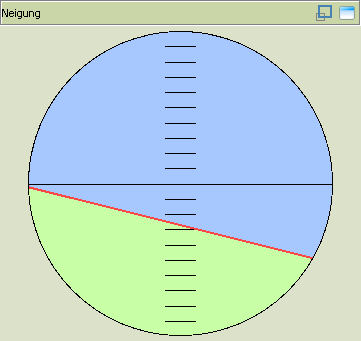
\includegraphics[width=.4\textwidth]{images/neigung}
	\caption{Das Neigungs-Plugin}
	\label{img:plugins:neigung}
\end{figure}

\section{Laserentfernungsmesser}
\index{Laserentfernungsmesser}
Dieses Plugin zeigt Scans eines Laserscaners an. Aus einem solchen Scan
resultiert eine grober Umriss der Umgebung. Die F�llfarbe kann gew�hlt werden.
Eine weitere Option ist, einen Rand um den Umriss zeichnen zu lassen. In
Abbildung \ref{img:plugins:laser} auf Seite \pageref{img:plugins:laser} ist das
Plugin in Aktion zu sehen.

\begin{figure}[htp]
	\centering
	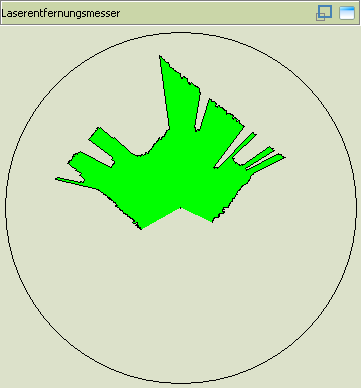
\includegraphics[width=.4\textwidth]{images/laser}
	\caption{Das Laserentfernungsmesser-Plugin}
	\label{img:plugins:laser}
\end{figure}

\section{Nachrichten}
\index{Testerbot}
\index{Sprachausgabe}
\index{Kommandos}
Das Nachrichten-Plugin zeigt die vom \seegls{Testerbot} erzeugten S�tze an. Ist die
Sprachausgabe aktiviert, werden diese S�tze (alle in englischer Sprache) �ber
das Sprachausgabesystem ausgegeben. Des Weiteren exportiert dieses Plugin eine
Funktion, welche mittels der Kommandos aufgerufen werden kann. Wird dieser
Funktion eine Taste zugewiesen, kann durch Dr�cken dieser Taste der Inhalt des
Textfensters gel�scht werden.

\section{Testerbot Protokoll}
\index{Testerbot}
\index{Datenpool}
Das \seegls{Testerbot} Protokoll verarbeitet die vom \seegls{Server} gesendeten Pakete und spielt
die Daten unter den korrekten Schl�sseln in den Datenpool\footnote{F�r weitere
Informationen �ber den Datenpool, lesen sie den
\href{\devguideurl}{Developer Guide}.} ein.

\section{IP Kommunikation}
\index{TCP/IP}
\index{Testerbot}
Dieses Kommunikationsmediumsplugin kann verwendet werden, wenn mit dem Roboter
via \seegls{TCP/IP} kommuniziert werden soll. Der \seegls{Testerbot} kann ausschlie�lich mit
diesem Medium angesprochen werden.
\par
\index{IP-Adresse}
In den Einstellungen ist es m�glich die \seegls{IP-Adresse} und den Port des
Roboters/\seegls{Server}s einzugeben. Die \seegls{IP-Adresse}n werden in IPv4 angegeben.

\section{Serielle Kommunikation}
\index{RS232}
Dieses Plugin realisiert eine Kommunikation �ber eine serielle Schnittstelle
(RS232). In den Einstellungen kann die zu benutzende Schnittstelle definiert und
konfiguriert werden.

\section{Carmen Kommunikation}
\index{Carmen}
\index{Carmen!IPC}
\index{Carmen!Carmen IPC Central Server}
Mit diesem Plugin l�sst sich eine Verbindung zu einem \seegls{Carmen} \seegls{IPC} Central \seegls{Server}
herstellen und Nachrichten an diesen verschicken. In den Einstellungen lassen
sich \seegls{IP-Adresse} und Port des \seegls{Server}s angeben.

\index{Plugins|)}
